Po desce o masie \emph{M}, leżącej na doskonale gładkich podporach pod kątem \emph{$\alpha$} do poziomu, biegnie stonoga o masie \emph{m}. Z~jakim przyspieszeniem i w którą stronę powinna biec stonoga, aby deska nie ześlizgnęła się z~podpór?
\begin{figure}[H]
	\centering
	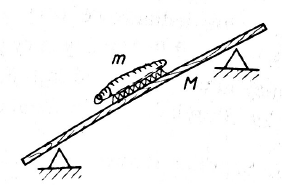
\includegraphics[width=0.3\linewidth]{../rysunki/dynamika/stonoga1.png}
\end{figure}

%Kruczek 9-18R/84
%Poziom C
